\chapter{Výsledky}

\section{Testovanie}
Pri testovaní vizualizácie sme postupovali podľa článku od Elmqvist et al. \cite{Patterns}, ktorý opisuje najpoužívanejšie vzory testovania vizualizácie a článok od Vogel et al., v ktorom autori testujú webovú vizualizáciu \cite{WebBasedUserTest}.

\subsection{Testovacia procedúra}
Testovanie prebiehalo v dvoch častiach prostredníctvom niekoľkých úloh, ktoré sme navrhli na základe špecifikácie požiadaviek na vizualizáciu uvedených v sekcii \ref{sec:spec}.

V prvej časti sme testovali náš systém a v časti druhej starý používaný spôsob pozostávajúci z čiarových diagramov pre jednotlivé mesiace v roku (pozri prílohu \ref{sec:oldsys}).

V oboch častiach bola každému testovaciemu subjektu vysvetlená podstata verifikácie a predstavená základná funkcionalita systému v krátkom 15 minútovom návode. Následne subjekt obdržal testovací formulár (pozri prílohu \ref{sec:testform}) obsahujúci 7 rôznych úloh, ktoré mal subjekt vykonať a po vykonaní každej z nich do formulára zapísať výsledok svojho skúmania.

Jednotlivé časti testovania boli vykonané následne za sebou na rovnakých testovacích subjektoch. Teda po testovaní prvého systému rovnaký subjekt testoval druhý systém.

Pri testovaní sme jednak skúmali správnosť odpovedí ale aj rýchlosť vykonania jednotlivých úloh.

\subsection{Testovacie dáta}
Na testovanie sme použili reálne dáta predpovedí modelu \textbf{WRF} pokrývajúce celý Arabský poloostrov a pozorovania (merania) z konkrétnych meteorologických staníc v meste Dubaj.

Keďže sme robili porovnávacie testovanie dvoch systémov s rovnakou množinou užívateľov, rozhodli sme sa pre rôzne systémy použiť rôzne dáta. Takýmto spôsobom sme sa snažili vylúčiť to, že subjekt použije už naučené poznatky z predošlého pokusu, keďže našou snahou bolo získať, čo najpravdivejšie výsledky testovania. 

Náš systém sme testovali na predpovediach \textit{tlaku} z roku \textit{2012} pre Dubajskú stanicu \textit{Al Faqa}, zatiaľ čo starý systém sme testovali na predpovediach \textit{teploty} z roku \textit{2013} pre stanicu \textit{Jebel Ali}. Použili sme teda dáta pre rozdielnu veličinu, rok a stanicu.

\subsection{Výsledky testovania}

Vizualizáciu sme testovali na 6 subjektoch bez vyššieho meteorologického, matematického alebo informatického vzdelania. Taktiež žiaden užívateľ nemal skúsenosti s verifikáciou predpovedí a náš systém videl prvýkrát v živote. Všetky tieto faktory vplývali na výsledok nášho testu, keďže sme sa často stretali s nepochopením, respektíve s pomalým pochopením zadania a teda čas riešenia úlohy sa značne natiahol.

\begin{table}[h]
	\centering
	\caption{Výsledky testovania}
	\label{table:results}
	\begin{tabular}{|c|c|c|c|c|}
		\hline
		\rowcolor[HTML]{9B9B9B} \textbf{Úloha} & \textbf{Systém 1} & \textbf{Systém 2} & \textbf{Priemerný čas 1} & \textbf{Priemerný čas 2} \\ \hline
		1  &  6/6   &  3/6 	 &  23.85s 		    &  44.81s   \\ \hline
		2  &  6/6   &\textemdash&  37.27s 		    &  \textemdash   \\ \hline
		3  &  6/6   &  4/6   &  24.66s 		    &  \textbf{15.2s}   \\ \hline
		4  &  6/6   &  2/6   &  \textbf{40.36}s &  48.69s   \\ \hline
		5  &  6/6   &\textemdash&  24.69s          &   \textemdash   \\ \hline
		6  &  6/6   &  4/6   &  \textbf{9.73}s  &  73.37s   \\ \hline
		7  &  6/6   &  1/6   &  23.27s          &  \textbf{127.53s}   \\ \hline
		\rowcolor[HTML]{C0C0C0} \textbf{Suma}  & \textbf{42/42} & \textbf{14/30} & \textbf{183.83s} & \textbf{312.5s}\\ \hline
	\end{tabular}
\end{table}

\pagebreak

V tabuľke \ref{table:results} vidíme, že v našom systéme \mbox{(Systém 1)} boli všetci užívatelia stopercentne úspešný a teda všetky úlohy vyriešili správne. Avšak v starom systéme \mbox{(Systém 2)} bola úspešnosť len polovičná, pričom dve úlohy nebolo možné vyriešiť pomocou danej vizualizácie vôbec.

Rovnako aj v nameraných časoch bol náš systém výrazne lepší. Celkový čas potrebný na riešenie siedmich úloh zabral testovaným užívateľom v priemere 3 minúty, a vykonanie jednej zabralo v priemere asi pol minúty (26s), zatiaľ čo v starom systéme vyriešenie piatich úloh trvalo vyše 5 minút a každá úloha zabrala v priemere asi 1 minútu (62s).

V tabuľke sme tiež zvýraznili najdlhší a najkratší priemerný čas z vykonávaných úloh. Vidíme, že úloha, ktorá bola v našom systéme očividne najjednoduchšie riešiteľná, mala v starom systéme druhý najhorší priemerný čas. Avšak úloha, ktorá zabrala v našom systéme najviac času, trvala podobný (aj keď o niečo lepší) čas ako pre starý systém, nehladiac na to, že riešenie úlohy v starom systéme bolo pomerne neúspešné a to iba 2 z 6 subjektov odpovedalo správne. Lepšie porovnanie jednotlivých časov pre dané úlohy môžeme vidieť v grafe na obrázku \ref{fig:times}.

Ak by sme mali zhodnotiť náš systém v porovnaní so starým na základe výsledkov testovania, môžeme povedať, že riešenie jednotlivých úloh analýzy dát je v našom systéme pomocou nami navrhnutej vizualizácie výrazne jednoduchšie a presnejšie.

\begin{figure}
	\centering
	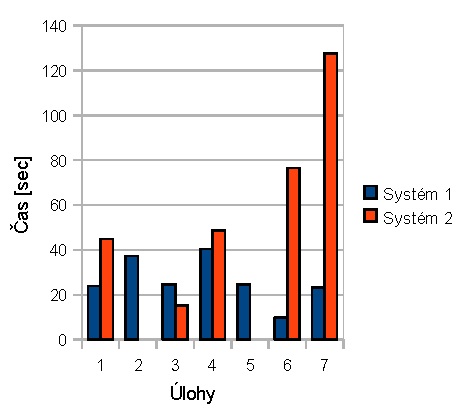
\includegraphics[width = 3in]{times}
	\caption{Porovnanie časov nášho (Systém 1) a starého systému (Systém 2)}
	\label{fig:times} 
\end{figure}

\subsubsection{Zhodnotene výsledkov nášho systému}
V grafe na obrázku \ref{fig:results} môžeme lepšie vidieť sumárne porovnanie časov pre jednotlivé úlohy a užívateľov. Ľahko sa dá všimnúť, že úlohy 1, 2, 5 a 7 majú približne rovnaký priemerný čas, zatiaľ čo úlohy 2, 4 mali výrazne dlhšie trvanie a úloha 9 trvala v priemere najkratšie.

Dlhé trvanie úlohy 2 prisudzujeme vyššej zložitosti úlohy oproti ostatným. Pre užívateľov bolo odhalenie outlierov pomerne rýchle, avšak väčšinu času zabralo užívateľom odčítanie z grafu o akú presnú hodnotu a predpoveď ide.

Pri úlohe 4 bolo problémom rýchle odčítanie z grafu, o aký dátum sa jedná. Dôvodom bolo nedobré označenie dátumov na \mbox{$ x $-ovej} škále, kedy sa jednotlivé dni v roku označujú číslami 0-364. Užívateľ uvidel konkrétny dátum až keď nadišiel myšou na dané miesto, kedy sa mu presné hodnoty ukázali v \textit{tooltipe}. Lepším riešením by bola redšia škála s mesačnými intervalmi alebo konkrétnymi dátumami.

Výsledky nášho testovania považujeme celkovo za uspokojivé, keďže aj neskúsení užívatelia dosahovali pri všetkých úlohách dobré časy. Taktiež nám tieto výsledky poukázali na slabiny našej práce, ktorými sú hlavne zlé alebo slabé označenia škál, grafov a legiend.


\begin{figure}
	\centering
	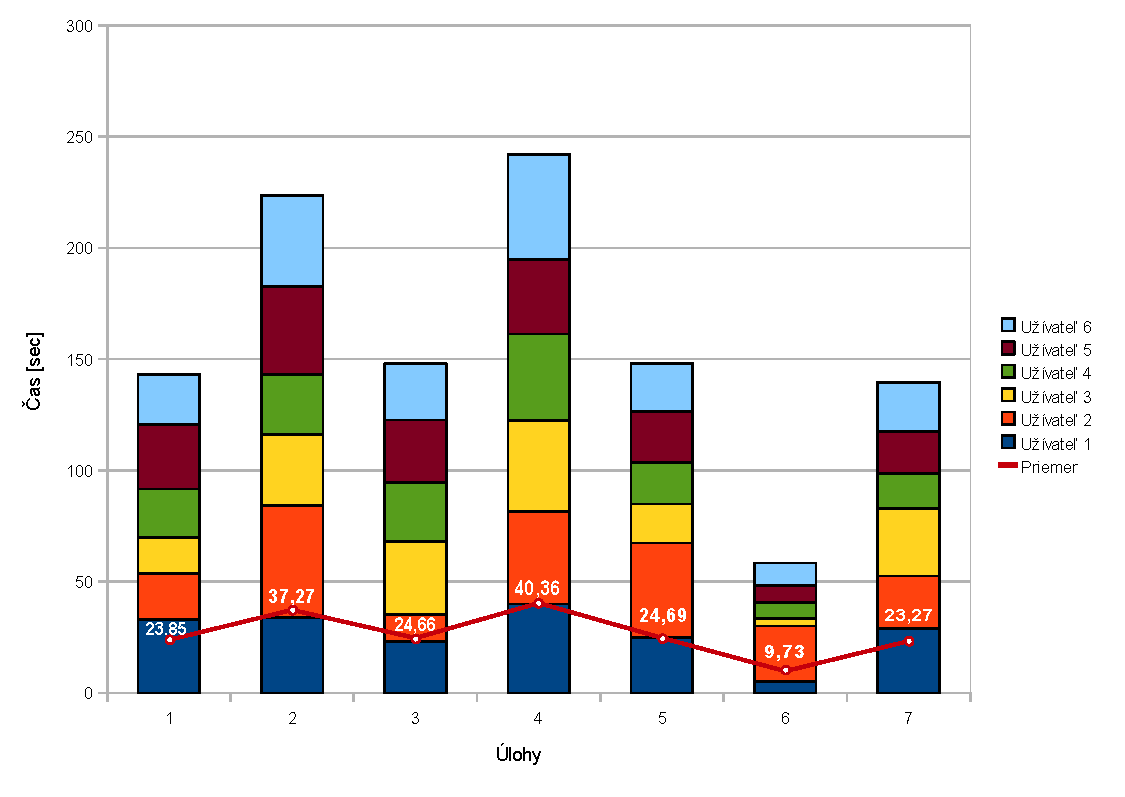
\includegraphics[width = 4in]{resultchart}
	\caption{Výsledky testovania nášho systému pre jednotlivých užívateľov.}
	\label{fig:results} 
\end{figure}

\section{Demonštrácia}
V tejto časti chceme demonštrovať príklad analýzy fungovania predpovedného modelu pomocou nami navrhnutých techník vizualizácie. Rovnako ako pri testovaní vizualizácie aj tu sme použili predpovedané dáta z modelu WRF. Konkrétne sa jednalo o tlak pri povrchu zeme v hektopaskaloch.

\subsection{Štatistiky}
Na obrázku \ref{fig:overview}a môžme vidieť farebnú mapu (Prehľad) zobrazujúcu RMSE pre celý rok 2012. Ako už vieme zo sekcie \ref{sec:errormeasurement}, RMSE nadobúda iba kladné hodnoty a teda nehovorí nič o smeru chyby, ale iba o jej veľkosti. 

Z daného obrázka ľahko vyčítať niektoré zaujímavé vzory. Ku príkladu je veľmi dobre vidno, že model predpovedá najlepšie v okolí šiestej hodiny predpovede a v okolí poludnia zaznamenávame prudký pokles presnosti predpovedí. Fakt, že model predpovedá najlepšie až okolo šiestej hodiny a nie ihneď na začiatku predpovede trocha nabúra náš predpoklad, že smerom do budúcnosti sa predpoveď zhoršuje. Tu sa potvrdzuje dôležitosť vizualizácie, ktorá slúži nielen na to, aby sme \textit{zistili očakávané}, ale aj \textit{objavili neočakávané}.

Na obrázku \ref{fig:overview}b máme zobrazenú priemernú chybu (MFE), ktorá sa počítala z rovnakých dát ako RMSE na obrázku \ref{fig:overview}a. Na tomto grafe je ihneď vidieť to, či model podhodnocuje alebo nadhodnocuje predpovede. Ako vidíme väčšina grafu je zafarbená na modro, čo značí záporné hodnoty, a teda podhodnotenie predpovedí. Taktiež vďaka dobre zvolenej farebnej škále môžeme vidieť, že niektoré hodnoty (napríklad 6 hodina v Januári) sú kladné, avšak stále blízko nuly.

\begin{figure}
	\centering
	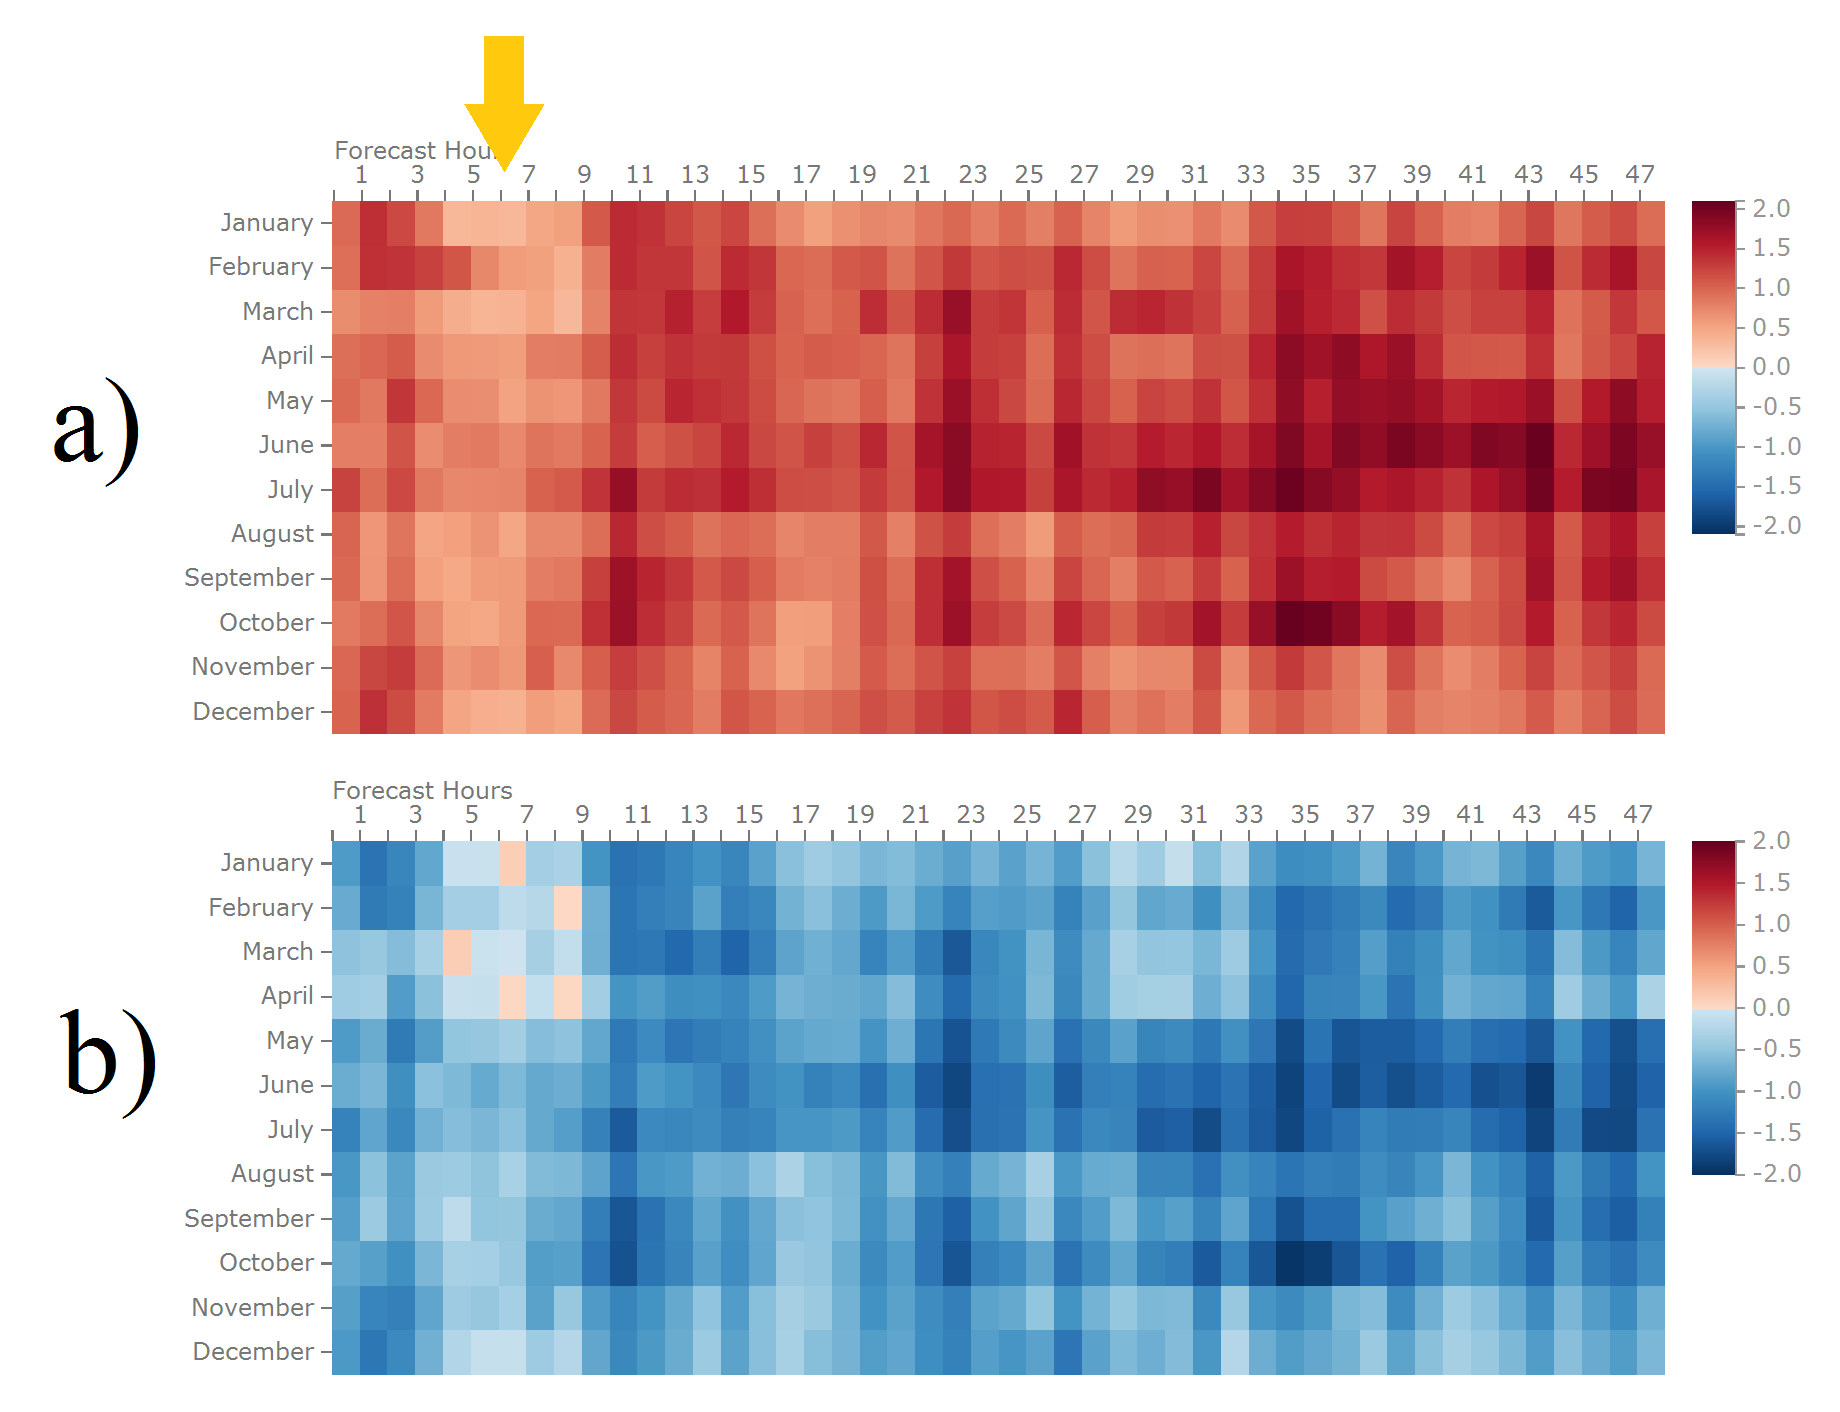
\includegraphics[width = 5in]{overview}
	\caption{a) Farebná mapa zobrazujúca RMSE b) Farebná mapa zobrazujúca MFE}
	\label{fig:overview} 
\end{figure}

V prípade, že užívateľ potrebuje získať informáciu o veľkosti a aj smere chyby súčasne, po kliknutí na konkrétny mesiac sa mu zobrazia všetky vypočítané štatistiky súčasne (pozri obrázok \ref{fig:detail}). O aké štatistika sa jedná vidíme v \textit{tooltipe} podľa farebného rozlíšenia.

\begin{figure}
	\centering
	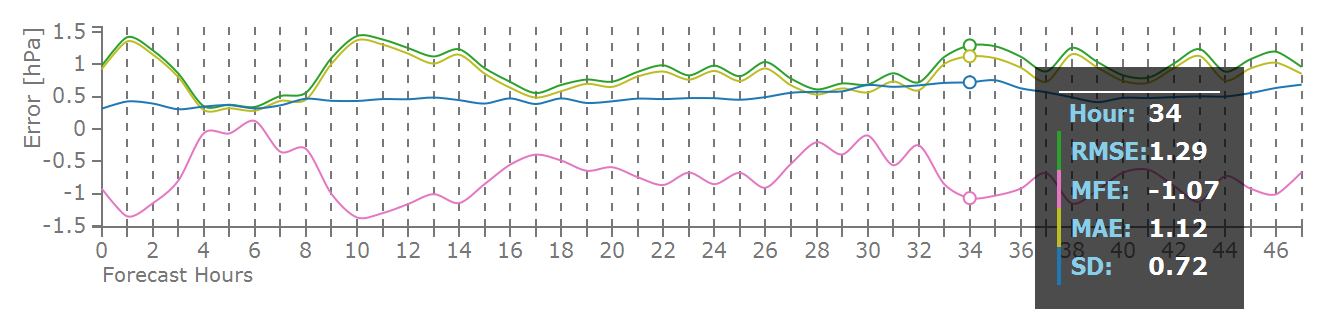
\includegraphics[width = 6in]{detail}
	\caption{Zobrazenie RMSE, MFE, MAE a SD (Standard Deviation) na jednom grafe súčasne}
	\label{fig:detail} 
\end{figure}


\subsection{Chyby}

Súčasťou obrazovky vizualizácie je aj zobrazenie jednotlivých chýb, z ktorých sa počítali štatistiky, či už pomocou farebnej mapy alebo pomocou grafov pre vizualizáciu distribúcie chyby.

Farebná mapa na obrázku \ref{fig:errors} nám dáva dobrý obraz o chybách v chronologicky zoradených predpovediach pre mesiac Február. Na tomto grafe si môžeme všimnúť niektoré predpovede, ktoré boli celkom úspešné - napríklad predpovede 4,5 a 12 majú chyby pomerne blízko 0, ale aj predpovede, ktoré sa nejakým spôsobom odlišujú od ostatných. Napríklad väčšina predpovedí podhodnocuje v hodinách 23-31, zatiaľ čo predpoveď 8 a 13 nadhodnocuje. Ďalej vidíme, že predpoveď 13 v okolí štvrtej hodiny má výrazný výkyv hodnôt a predpoveď 2 celkovo výrazne podhodnocuje.

Tento typ vizualizácie odporúčame kombinovať s jedným z grafom distribúcie, ktoré sú na obrázku \ref{fig:distrib}. Konkrétne na funkčnom krabicovom diagrame (obrázok \ref{fig:distrib}c) je veľmi dobre vidieť tri predpovede, znázornené červenou prerušovanou čiarou, ktoré sa výrazne líšia od ostatných. Sú to už spomínané predpovede 2, 8 a 13. Výrazný oblúk v okolí tretej hodiny patrí výkyvu hodnôt pre predpoveď 13, ktorý je ľahký objaviť aj v grafe na obrázku \ref{fig:errors}. Okrem tohto výkyvu nám graf ukazuje, že predpoveď 13 sa zvyšnou časťou krivky nachádza v centrálnej oblasti grafu, teda jej úspešnosť pre iné neskoršie hodiny je podobná ostatným predpovediam.

\begin{figure}
	\centering
	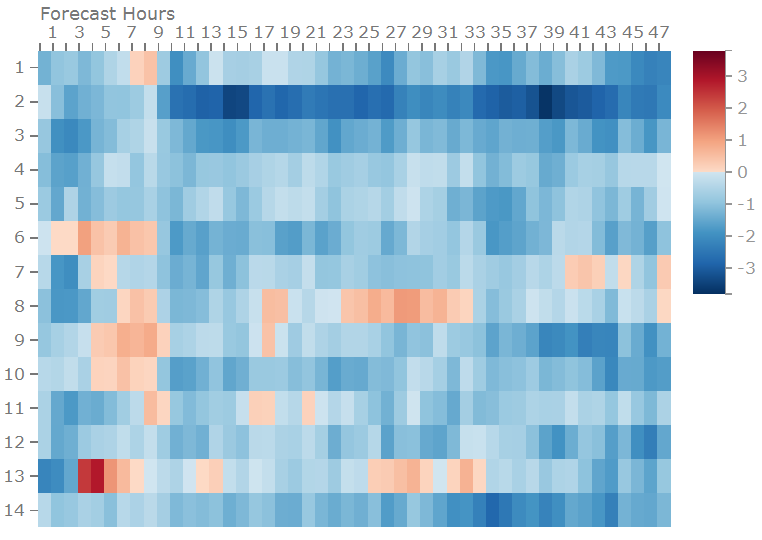
\includegraphics[width = 3.5in]{errors}
	\caption{Farebná mapa chýb predpovedí pre mesiac Február. Na \mbox{$ y $-ovej} osi je poradie predpovede.}
	\label{fig:errors} 
\end{figure}

Grafy na obrázkoch \ref{fig:distrib}a a \ref{fig:distrib}b nám podávajú rovnakú informáciu, avšak v rozdielnom detaile. Na oboch grafoch vidíme, že v okolí deviatej predpovednej hodiny majú chyby najmenší rozptyl. Vidíme aj, že v okolí štvrtej hodiny je naopak rozptyl väčší, avšak najväčšia hustota chýb sa stále nachádza blízko priemernej hodnoty, teda napriek výkyvom sú štatistiky z týchto dát pomerne dôveryhodné. Z grafu na obrázku \ref{fig:distrib}a možno vyčítať, že chyby pre niektoré hodiny majú už takmer bimodálnu distribúciu - druhá a posledná hodina predpovede.


\begin{figure}
	\centering
	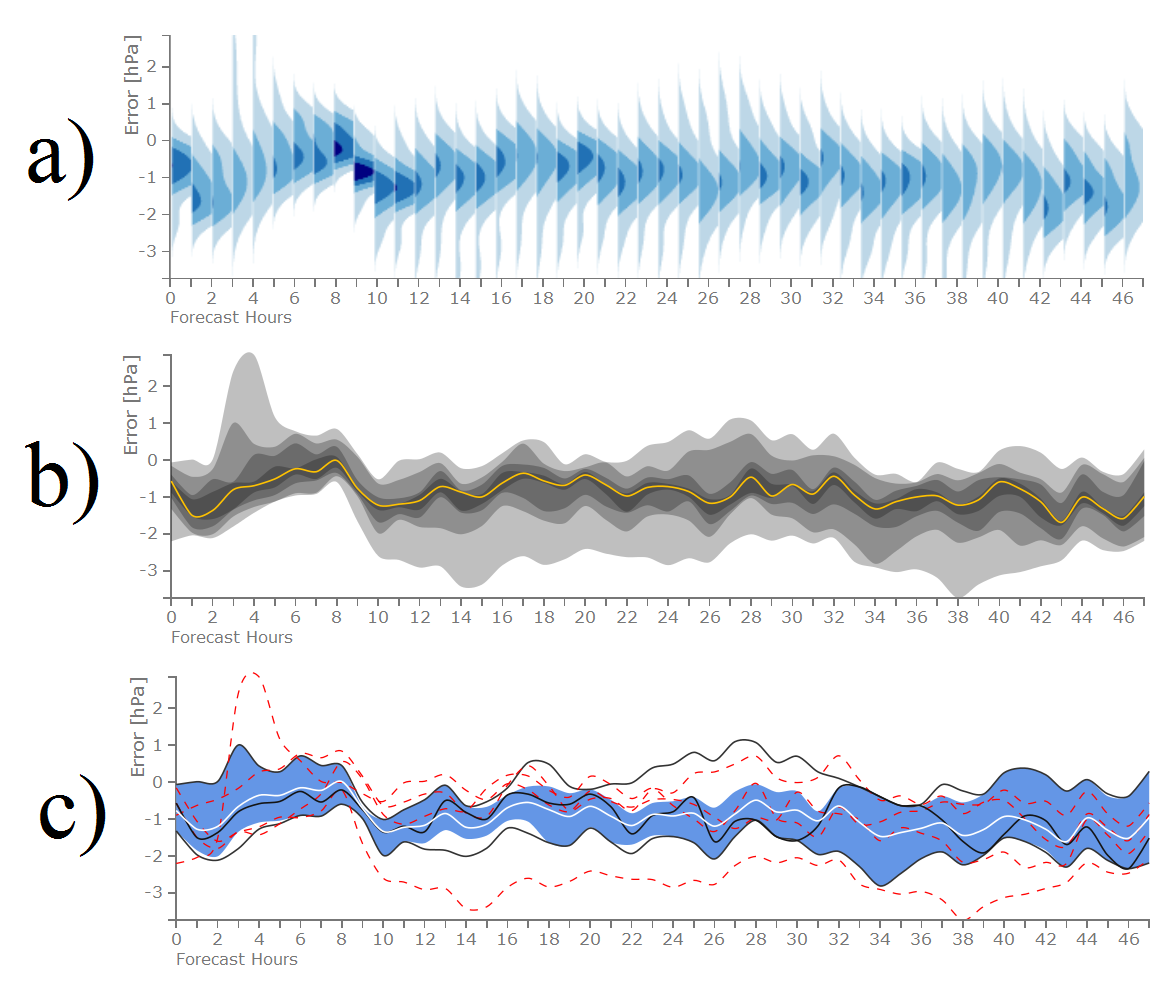
\includegraphics[width = 4in]{distrib}
	\caption{Grafy distribúcie pre mesiac Február a) Graf hustoty b) Pruhový kvantilový diagram c) Funkčný krabicový diagram}
	\label{fig:distrib} 
\end{figure}

\subsection{Ročný priebeh}
Posledným grafom, ktorý sa objavil na našej vizualizačnej obrazovke verifikácie je čiarový graf pre ročný priebeh chýb predpovedí (pozri obrázok \ref{fig:progress}). Na \mbox{$ x $-ovej} osi grafu máme jednotlivé dni v roku (0-364) a na \mbox{$ y $-ovej} veľkosť chyby v hPa. Tento graf zobrazuje denné štatistiky šedou čiarou a červenou je vyhladená táto krivka pomocou kĺzavého priemeru.

Na obrázku \ref{fig:progress} máme konkrétne RMSE. Celkovo vidíme, že v strede roka (v lete) sú chyby najväčšie a niekedy v novembri sú chyby najnižšie. Dôvodom však môžu byť aj chýbajúce dáta, keďže šedá krivka je podozrivo konštantná rovno na nule. Veľké skoky hodnôt môžeme pozorovať aj niekedy začiatkom februára, respektíve koncom januára a taktiež aj koncom decembra.


\begin{figure}
	\centering
	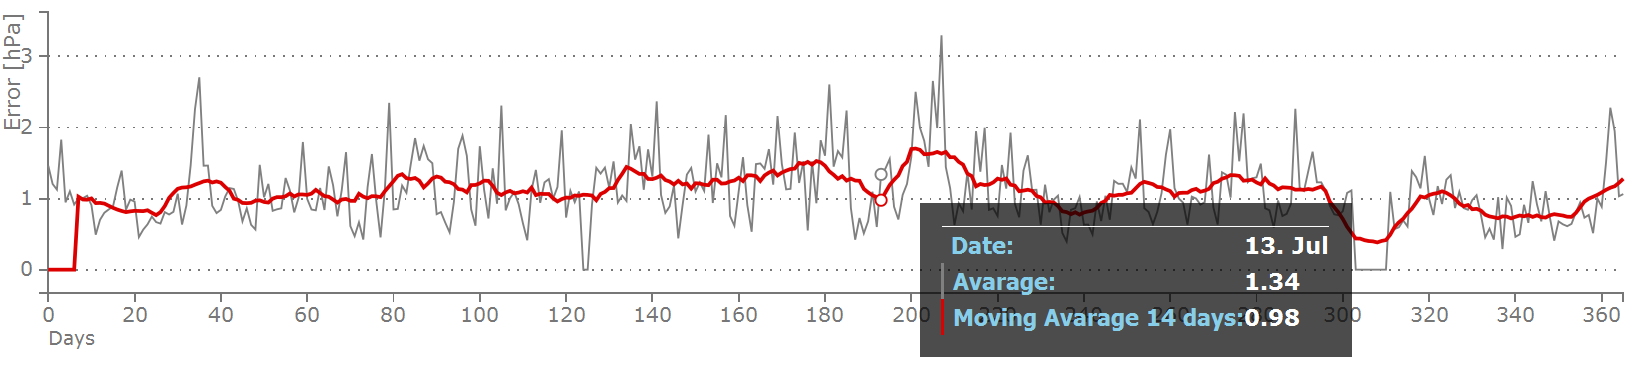
\includegraphics[width = 6in]{progress}
	\caption{Graf ročného priebehu chýb predpovedí. Šedou čiarou sú zobrazené denné štatistiky (konkrétne RMSE) a červenou je kĺzavý priemer vypočítaný z týchto štatistík. }
	\label{fig:progress} 
\end{figure}